% !TeX root = ../thesis.tex
\section{Background}
The background section will cover eight topics.
Section \ref{subsec:background:lifeinsurance} will explain insurance policies in general.
In section \ref{subsec:background:thielerungekutta} the mathematics employed in this project will be covered. 
This consists of Thiele's differential equation and the fourth-order Runge-Kutta method for solving differential equations.
Following this is a brief description of Diracs delta function.

After the mathematics is described, the technologies utilized will be presented.
General information on parallelization and the potential benefits of using the GPU compared to the CPU will be explained in section \ref{subsec:background:parallelization}.
The CUDA platform and CUDA C will then be presented in section \ref{subsec:background:cudac}.
In section \ref{subsec:background:codequotations} F\#'s meta-programming model Code Quotations is introduced.
Quotations are used to generate CPU code by the language-integrated compiler Alea.cuBase which will be presented in section \ref{subsec:background:fsharpcubase}.
Section \ref{subsec:cudaoptimization} will then briefly mention some approaches to CUDA optimization, namely occupancy and Instruction Level Parallelism.
Section \ref{subsec:background:calcspec} will briefly introduce the syntax of the Actulus Calculation Specification (CalcSpec).
In section \ref{subsec:background:hardware} the hardware the project has been tested on will be presented.

\subsection{Life Insurance Policies and the Markov-model}\label{subsec:background:lifeinsurance}
A life insurance policy is a contract stating the obligations an insuring party has to an insured party, in and transitioning between a finite set of states over many years.
Such states can include being alive and well (active), disabled, dead and more.
Transitions between states will have a certain probability, for example mortality rates for transitions between the active and dead state.
A state model such as this is also known as a continuous-time Markov-model\cite{norberg2000basic} which is used for both its expressiveness and its analyzability.

Figure \ref{fig:markovexample} shows an example of such a model with three states and three transitions between states. 
The labels between the states each have a $\mu$-function that states the probability of the transition occurring at time $t$. 
This is also known as the transition intensity.
Not all transition intensities will change over time while others such as mortality rate will.
For each change in time there may be associated costs whether there is a state transition or not.

\begin{figure}[H] 
\setlength{\unitlength}{0.14in} % selecting unit length 
\centering % used for centering Figure 
\begin{picture}(20,8) % picture environment with the size (dimensions) 
 % 32 length units wide, and 15 units high. 
\put(3,6){\framebox(6,3){0 (Active)}} 
\put(13,6){\framebox(6,3){1 (Disabled)}}
\put(8,0){\framebox(6,3){2 (Dead)}} 

\put(6.2,6){\vector(1,-1){2.9}}
\put(9,7.5){\vector(1,0){3.9}} 
\put(16.2,6){\vector(-1,-1){2.9}}

\put(9.5,8.5) {$\mu_{01}(t)$}
\put(15,4) {$\mu_{12}(t)$} 
\put(4.5,4) {$\mu_{02}(t)$} 
\end{picture} 
\caption{Disability Term Insurance Markov-model example} % title of the Figure 
\label{fig:markovexample} % label to refer figure in text 
\end{figure} 

\subsubsection{Example life insurance policies}\label{subsubsec:background:insuranceplans}
The following six life insurance plan examples are used throughout the project.
\begin{itemize}
\item Pure Endowment : The ensurer pays a lump sum if the ensured dies before age of retirement. 
\item $m$-year Deferred $n$-year Temporary Life Annuity : After $m$ years, ensurer makes yearly payments to the ensured for $n$ years given the ensured is alive.
\item $n$-year Temporary Life Annuity Premium : The ensured is paid yearly for $n$ years if alive.
\item $n$-year Term Insurance : The ensurer pays a lump sum if the ensured dies before $n$ years.
\item Disability Annuity : The ensured is paid yearly for $n$ years if disabled.
\item Disability Term Insurance : The ensurer pays a lump sum upon disability of ensured if it happens within $n$ years.
\end{itemize}

\subsection{Thiele's differential equation and the Runge-Kutta Method}\label{subsec:background:thielerungekutta}
The goal of the computations performed in this thesis is to estimate the amount of money (reserve) required to be able to fulfil the obligations of a given life insurance plan.
Thiele's differential equation called ``\emph{the foundation of modern life insurance mathematics}''\cite{bergermathematik} is a tool for determining conditional expected values in Markov models and it can be used to express a variety of life insurance policies.
The equation is expressed below in equation \ref{eq:thiele}. It assumes continuity for $V_s$, $b_s$, $\mu$ for every $t$ and consists of the following parts:

\begin{itemize}
\item $s$ is the state
\item $V_s(t)$ is the reserve at time $t$ in state $s$
\item $r_s(t)$ is interest-rate at time $t$ in state $s$
\item $b_s(t)$ is the benefit paid by the insurer at time $t$ in state $s$
\item $T_s$ is the set of states which can be transitioned to from state $s$
\item $\mu_{s,ts}(t)$ is the transition intensity from state $s$ to state $ts$
\item $b_{s,ts}(t)$ is the transition cost from state $s$ to state $ts$
\end{itemize}

\begin{equation}\label{eq:thiele}
\frac{d}{dt}V_s(t) = r_s(t) V_s(t) - b_s(t) - \sum_{ts \in T_{s}} \mu_{s,ts}(t) (V_{ts}(t) - V_s(t) + b_{s,ts})
\end{equation}

To shortly summarize it, the change in reserve at time $t$ in state $s$ is the current reserve times the interest-rate minus the benefit paid by the ensurer in the state minus the weighted transitioning costs to all connected states. 
The weighted transitioning cost to a state is the intensity of the transition (probability of the transition occurring) times the difference in reserves plus the transitioning cost.
This results in the expected reserve of a state at time $t$.

With a differential equation such as this, one way to solve it is to approximate the result numerically using the Runge-Kutta method\cite{press2007numerical}.
The Runge-Kutta method is a method for integrating ordinary differential equations (ODEs) by using a trial step at the midpoint of an interval to cancel out lower-order error terms.
It works within boundaries set by a starting and end point. 
If the starting point is greater than the end point, the algorithm works backwards with negative step-sizes.
The basic implementation uses a fixed number of steps to reduce the inaccuracy of the method. 
By increasing the number of steps, the inaccuracy of the method is reduced at the cost of increased computational costs.
The most common step size seen in this project is 100 steps by advice of Peter Sestoft and by calculation specification definitions.
The fourth-order version of the Runge-Kutta method can be seen below in equation \ref{eq:rk4} approximating the equation-result $y$ in the step from $t$ to $t+h$. It consists of the following parts:

\begin{itemize}
\item $h$ is the size of the step. With 100 steps, the step-size would be 0.01, or -0.01 if the start point is greater than the end point.
\item $f(t, e)$  is the right hand side of the given differential equation evaluated at time $t$ in environment $e$
\item $t$ is the initial time of the step
\item $y_t$ approximated result at time t
\item $O(h^5)$ represents the maximal error of the method
\end{itemize}

\begin{equation}\begin{aligned}\label{eq:rk4}
&k_1 = h f(t, y_t)\\
&k_2 = h f(t + \frac{h}{2}, y_t + \frac{k_1}{2})\\
&k_3 = h f(t + \frac{h}{2}, y_t + \frac{k_2}{2})\\
&k_4 = h f(t + h, y_t + k_3)\\
&y_{n+1} = y_t + \frac{k_1}{6} + \frac{k_2}{3} + \frac{k_3}{3} + \frac{k_4}{6} + O(h^5)
\end{aligned}\end{equation}


\subsection{Dirac Delta Function}\label{subsec:delta}
The Dirac delta function, or $\delta$ function, is not strictly a function but is a distribution on the real number line that is zero everywhere except at zero with an integral of one over the entire real line.
It is used in actuary science to model ``sudden shocks'', or lump sum payments, but is not very commonly seen in computing.
The method has many restrictions that apply and should primarily be of the form \lstinline$factor * delta(constant - variable)$ where $factor$ is constant and represents the ``sudden shock'' that should occur when \\\lstinline$constant - variable = 0$.
%Insert graphics showing step

\subsection{Parallelization and the GPU}\label{subsec:background:parallelization}
Parallelization is the act of taking one large task and splitting it into smaller tasks that run concurrently (``in parallel'').
This could for example be cooking ten different pies, where rather than using one baker you now use ten bakers creating ten pies at the speed of one.
Algorithmically this could be an algorithm that initially does some computation that loops $n$ times where each iteration is independent and takes $w$ time to complete, but is altered to instead utilize $n$ tasks that each execute one iteration worth of work.
Instead of taking $w \cdot n$ time to complete, it can now be done in just $w$ time plus whatever overhead is associated with creating the tasks and dividing the work.
This is reliant on each iteration being independent, as if the iterations are dependent on each other then an iteration can not be executed before the prior iteration completes.
To continue the pie example, if one baker is assigned to make all the pie-crusts, no pie will be baked before this task is done.
Loops are not the only thing that can be parallelized and all independent tasks can to some extend be parallelized. 
With various synchronization techniques, partially dependent calculations can also harness the power of parallelization, though at the risk of increased complexity and errors such as deadlocks.
As only parallelization of independent computations are utilized, other forms will not be discussed further.

In computing, parallelization utilizing constructs such as processes and threads can be executed on multi-core CPUs, but can especially be used by GPUs that were designed for compute-intensive and highly parallel computations which is what graphics rendering is all about.
This is because unlike the CPU which is a general-purpose machine with a focus on data-caching and flow control, the GPU is specialized for powerful arithmetic processing with more transistors dedicated to data processing as illustrated in green by figure \ref{cpugpu}. 
The figure contains Arithmetic Logic Units (ALU's, in green) responsible for logical operations and integer arithmetic, Control Units (in yellow) responsible for communication and coordination between input/output devices and various memory units (in orange), such as a memory cache and dynamic random-access memory (DRAM).

\begin{figure}[H]
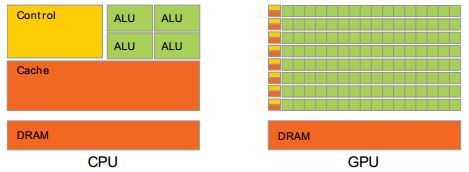
\includegraphics{cpugpu.jpg}
\caption{Structural comparison of the CPU and GPU.\label{cpugpu}}
\caption*{From the CUDA C Programming Guide, page 3 \cite{nvidia2014programming}}
\end{figure}

\subsection{The CUDA platform and CUDA C}\label{subsec:background:cudac}
CUDA is NVIDIA's parallel computing platform and programming model for the GPU.
It is available on multiple platforms but does require an NVIDIA graphics card. 
An NVIDIA graphics card will have a certain Compute Capability (CC) that determines availability of certain attributes and features.

The CUDA platform consists of the CUDA C and C++ language (referred to as CUDA C from this point), based on the C and C++ languages but with some alterations.
It also has parallel computing extensions for other languages such as Fortran and Python.
The CUDA Toolkit is also a part of the platform, consisting of a compiler, math libraries and tools for debugging and optimizing performance as well as guides, user manuals, API references and other documentation.

\subsubsection{CUDA Architecture}
The CUDA model is build around a hierarichal architecture of the GPU. 
At the top of the architecture is the streaming multi-processor (SM) of which a GPU can have many. 
Each SM consists of multiple CUDA cores that are used to concurrently execute a group of 32 threads known as a warp. 
As the SM executes the instructions in terms of warps, the total number of threads in a block should be a multiple of the warp-size for maximum efficiency.
Each SM executes one group of threads that have access to a shared memory-space.
This group of threads, which ideally should be a multiple of warps, is called a block. 
An example overview of the architecture can be seen in figure \ref{cuda_architecture}.
As each SM executes blocks sequentially, more SMs available to the GPU will increase the possible parallelization and speed up the execution of the total amount of blocks. 
Assuming that blocks will generally finish at the same time, this also means that the amount of blocks should be a multiple of the amount of multiprocessors for maximum efficiency.

\begin{figure}[H]\centering
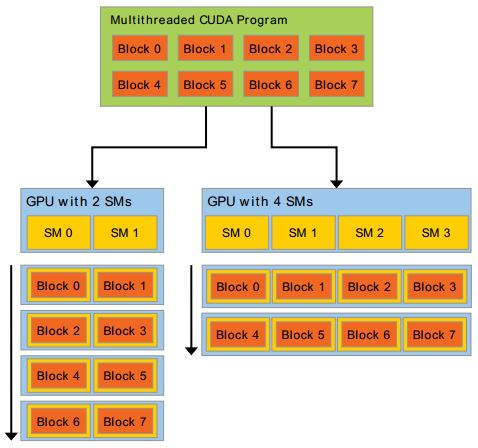
\includegraphics[scale=0.6]{cuda_architecture.jpg}
\caption{The CUDA SM/block architecture.\label{cuda_architecture}}
\caption*{From the CUDA C Programming Guide, page 7 \cite{nvidia2014programming}}
\end{figure}

\subsubsection{Thread Hierarchy}
Blocks can be organized in a grid of multiple dimensions (up to three on the latest version of NVIDIA cards). 
The same applies to the threads within a block.
An example of a thread hierarchy can be seen in figure \ref{thread_distribution}.

\begin{figure}[h!]\centering
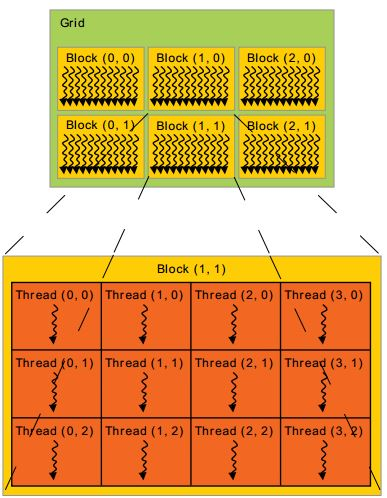
\includegraphics[scale=0.75]{thread_distribution.jpg}
\caption{The CUDA thread hierarchy.\label{thread_distribution}}
\caption*{From the CUDA C Programming Guide, page 11 \cite{nvidia2014programming}}
\end{figure}

As this project only utilizes one-dimensional grids and blocks, the resulting thread hierarchy is a two-dimensional matrix. 
An example with the unique thread-IDs can be seen in figure \ref{thread_hierarchy}.

\begin{figure}[h!]\centering
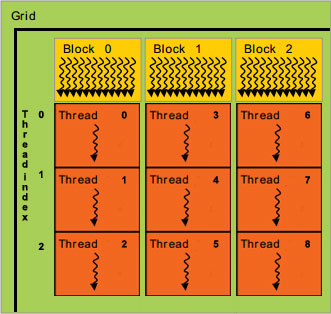
\includegraphics[scale=0.75]{thread_hierarchy.jpg}
\caption{CUDA thread hierarchy with one-dimensional blocks and threads.\label{thread_hierarchy}}
\end{figure}


\subsubsection{Memory model}
A GPU program (referred to as a kernel from here) has access to various types of memory.
There is \emph{local} memory only available to the thread itself.
This is facilitated by 32 kibibyte (KiB, which is 1024 bytes) per block of fast registers while available and falling back on relatively slow local memory afterwards which is stored in global memory but only accessed by the thread.
Each register holds up to four bytes.
Each CUDA thread can use at most 63 registers making 512 the highest warp-sized number of threads per SM.
If the kernel uses no more than 32 registers, up to 1024 threads per SM can be used.

Beyond that, it has access to up to 48KiB per block low-latency \emph{shared} on-chip memory physically residing on the GPU that is available to all threads in the same block. 
Because of these properties, shared memory can be used for communication between threads or as a software managed cache.

The thread also has access to \emph{global} off-chip memory accessible to all threads in all blocks.
This has a higher latency, but caching can alleviate some of this.

There is also 64KiB of immutable cached \emph{constant} memory which can be an alternative to unchanging global memory.
It is especially fast when all threads in the warp need to read the same memory location.
Constant memory will often be faster than global memory due to a higher likelihood of being cached on-chip, but the fact it is immutable and of a fixed size limits its applicability.
Another immutable memory type is \emph{texture} memory which can be used for various purposes, but is ideally used for algorithms with memory access patterns where threads are likely to read from an address that is 2-dimension-spatially local (such as computer graphic shaders).

Data loaded from local or global memory is cached in the on-chip \emph{L1} cache for each SM and a shared \emph{L2} cache for all SMs.
The L1 cache will typically contain up to 16KiB of data, but this limit can be increased by up to 48KiB by sacrificing shared memory size.
The L2 cache will on newer graphics cards contain up to 768KiB of data.
A summary of the properties of the various memory types can be seen in table \ref{table:memorytypes}.

\begin{table}[H]
\centering
{\setlength{\extrarowheight}{2pt}{\setlength{\tabcolsep}{3pt}
\begin{tabular}{ | c | c | c | c | c | }
  \hline
			&	Read-only	& On-chip	&	Cached	&	Scope	\\ \hline
Register	&	No			& Yes		&	No		&	Thread	\\ \hline
Local		&	No			& No		&	Yes		&	Thread	\\ \hline
Shared		&	No			& Yes		&	No		& 	Block	\\ \hline
Global		&	No			& No		&	Yes		&	Kernel	\\ \hline
Texture		&	Yes			& No		&	Yes		&	Kernel	\\ \hline
Constant	&	Yes			& No		&	Yes		&	Kernel	\\ \hline
L1 Cache	&	No			& Yes		& 	N/A		&	N/A		\\ \hline
L2 Cache	&	No			& No		&	N/A		&	N/A		\\ \hline
\end{tabular}}}
\caption{Properties of CUDA memory types\label{table:memorytypes}}
\end{table}

\subsubsection{CUDA C}
CUDA C is based on C and C++ with added declaration specifiers for methods and variables. 
The most essential declaration specifier is the \textbf{\_\_global\_\_} specifier which declares a method to be a \textbf{kernel}. 
Kernels are void-methods that are callable from the CPU but executed on the GPU. 
Code sample \ref{cuda_add} shows a simple kernel performing vector addition of the vectors $a$ and $b$ of size $N$.
%\clearpage
\begin{lstlisting}[language=cudac, caption=CUDA C addition kernel, label=cuda_add]
__global__ void Add(float *a, float *b, float *result){
	//unique id within the kernel
	int i = threadIdx.x + blockIdx.x * blockDim.x;
	// (blockIdx always 0 in this example)
	result[i] = a[i] + b[i];
}

int main(){
	...Initiate memory on host and device
	Add<<<1, N>>>(a, b, result); //run kernel on 1 block of N threads
	...Copy back and use result, free memory as appropriate
}
\end{lstlisting}

One thing to note is the kernel launch-parameters of the Add-method in $main$ which specify the number of blocks and the number of threads per block on which the kernel should be executed. 

CUDA C also has other declaration specifiers. 
The \textbf{\_\_device\_\_} specifier indicates that a method will only be compiled for the GPU which can be referenced by kernels, the \textbf{\_\_host\_\_} specifier indicates that a method will be available for the CPU.
These two specifiers can also be used together for compilation to both platforms.
If no specifiers are explicitly stated the \textbf{\_\_host\_\_} specifier is used.
Variables also have the \textbf{\_\_device\_\_} specifier indicating they should be stored on the device typically in global memory, as well as the \textbf{\_\_constant\_\_} specifier to indicate that they are to be stored in constant memory and the \textbf{\_\_shared\_\_} specifier for shared memory.

As it is based on C, dynamic memory must be allocated using $malloc$ and subsequently de-allocated by $free$.
These operations also have to be performed for the device memory using the equivalent $cudaMalloc$ and $cudaFree$.
One of the many benefits of using a modern language is avoiding tedious memory management like this, but at the loss of control that could potentially decrease performance.

\subsection{F\# and Code Quotations}\label{subsec:background:codequotations}
F\#\cite{fsharp} is an open source, cross-platform functional programming language originating from Microsoft that runs on the .NET platform.
Code Quotations is a language feature of F\# that allows one to dynamically generate abstract syntax trees from F\# expressions. 
It is used in particular to transform F\# to other languages such as SQL automatically. 
It can also be used to generate F\# code that can be evaluated. 
Code Quotations support both typed and untyped expressions using \lstinline$<@ ... @>$ and \lstinline$<@@ ... @@>$ respectively. 

For example, the expression \lstinline$<@ let plus5 n = n + 5 in plus5 @>$ is automatically translated into the abstract syntax tree in code sample \ref{quotationast}. 
As Quotations only support expressions, a let declaration can not exist on its own, hence returning the function at the end (in the $in$ part of the Quotation).
%\clearpage
\begin{lstlisting}[language=FSharp, caption=Abstract syntax tree for the example Quotation expression, label=quotationast]
Let(plus5, Lambda(n, Call(None, op_Addition, [n, Value(5)])), plus5)
\end{lstlisting}

Code Quotations also allow for the mixing of Quotation expressions using the splicing operators $\%$ for typed and $\%\%$ for untyped expressions as can be seen in code sample \ref{quotationsmixin}.

\begin{lstlisting}[caption=Quotation mixing, label=quotationsmixin, language=FSharp]
let plus5:Expr<int->int> = <@ let plusfive n = n + 5 in plusfive @>
let plus10:Expr<int->int> = <@ let plusten n = n |> %plus5 |> %plus5 in plusten @>
let untypedplus10:Expr = <@@ %plus10 @@>
\end{lstlisting}


\subsection{F\# and Alea.cuBase}\label{subsec:background:fsharpcubase}
Alea.cuBase by QuantAlea\cite{quantalea} is a commercial language-integrated compiler for F\# that allows for CUDA development on the .NET platform.
By relying on runtime code generation it allows for very extensible kernels to an extent not easily possible in CUDA C.

It utilizes F\#'s meta-programming feature Code Quotations for automatic run-time generation of abstract syntax-trees that are then compiled into CUDA's Instruction Set Architecture (ISA) Parallel Thread Execution (PTX) code using Alea.cuBase's compilation API.
See figure \ref{fig:alea_cuBase_compilation} for an overview of the entire compilation process. %explain better

\begin{figure}[h!]\centering
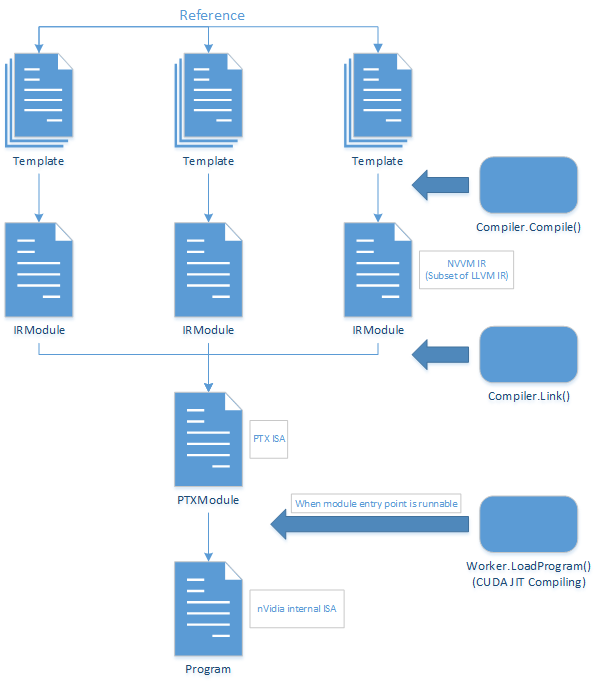
\includegraphics[scale=0.6]{cuBase_compilation_phases.png}
\caption{Phases of Alea.cuBase kernel compilation.\label{fig:alea_cuBase_compilation}}
\caption*{From the Alea.cuBase Manual 1.2.692\cite{quantalea}}
\end{figure}

Code sample \ref{cubase_add} shows what a simple vector squaring-kernel could look like in F\# using Alea.cuBase.

\begin{lstlisting}[caption=Alea.cuBase square kernel, label=cubase_add, language=FSharp]
let Square = cuda { //use the Alea.cuBase cuda workflow
  let! kernel = <@ fun (a:deviceptr<int>) (result:deviceptr<int>) ->
      let i = blockIdx.x * blockDim.x + threadIdx.x
      result.[i] <- a.[i] * a.[i] @> |> Compiler.DefineKernel
  return Entry(fun program ->
    let worker = program.Worker
    let kernel = program.Apply kernel
    //return host-execution method
    fun (a:int[]) ->
      use a = worker.Malloc(a)
      use result = worker.Malloc(Array.zeroCreate a.Length)
      kernel.Launch (LaunchParam(1, a.Length)) a.Ptr result.Ptr
      result.Gather()) //return result
}
[<EntryPoint>]
let main argv = 
  let a = [| for i in 1 .. 10 -> i |]
  use program = Square |> Compiler.load Worker.Default
  program.Run a |> Array.iter (fun e -> printfn "%d" e)
  0 //program success exit code
\end{lstlisting}

The $cuda$ workflow/computation expression (or monad) contains the kernel defined in a Code Quotation and compiled to an actual kernel, and it returns a host-side execution method that will handle allocation and de-allocation of device-side memory. 
As this thesis uses F\#, the deallocation is handled automatically by using the $use$-keyword that frees up resources once the variables referencing them are out of scope. 
The kernel is loaded to a worker (a CUDA context and background-thread) in the main method compiling the PTX code to NVIDIA internal ISA code and producing a runnable $Program$. 
Following this, the compiled kernel is run using the parameters defined in the kernel-invocation method of the $cuda$ workflow (in this case, just an integer array) and the result is returned to the CPU where it can be processed. 
In this example is it simply printed to the console. 


\subsection{CUDA Optimization}\label{subsec:cudaoptimization}
\subsubsection{Occupancy}\label{subsubsec:occupancy}
Occupancy is a term used to describe the ratio between the active and maximum active warps for a kernel.
It is a useful concept, as in order to hide latency from context switches on the GPU, the memory bus needs to be saturated by having enough transactions in flight.
To increase the number of transactions either the occupancy or the instruction level parallelism (see section \ref{subsubsec:ilp}) should be increased.

Things that potentially limit occupancy is register usage, shared memory usage and the number of threads per blocks.
To calculate thread occupancy, NVIDIA has provided a spreadsheet\cite{occupancycalculator} that calculates the occupancy percentage by taking the following parameters:
\begin{itemize}
\item Compute capability - which determines the following options
\item Total shared memory in bytes available
\item The number of threads per block
\item The number of registers per thread
\item Shared memory used per block in bytes
\end{itemize}

It is often not beneficial to have 100\% occupancy as long as enough transactions are in flight\cite{volkovoccupancy}.
Anecdotal evidence suggests around 66\% occupancy to be adequate for many situations (section 10.4 of the CUDA C Best Practices Guide\cite{cudacoccupancy}).


\subsubsection{Instruction Level Parallelism}\label{subsubsec:ilp}
Instruction level parallelism (ILP) is a term that covers the number of instructions relative to the number of dependent instructions when using parallel execution.
For example, consider the program seen in code sample \ref{ilpexample}.
The first two instructions are not dependent on each other and can be executed simultaneously.
If each operation can be completed in one unit of time, then these three instructions can be completed in two units of time for an ILP of $\frac{3}{2}$.

\begin{lstlisting}[caption=ILP example program, label=ilpexample]
a = b + c
d = e + f
g = a * d
\end{lstlisting}

It is no trivial task to increase ILP generally nor for the Runge-Kutta four solver and no particular work has been done to increase ILP for any of the solutions in this project.
Further work could ideally focus on increasing the ILP, as it could have a greater effect than increasing occupancy\cite{volkovoccupancy}.
It is likely that the memory bandwidth is saturated at higher kernel launch parameter configurations, so assuming that the typical use case includes hundreds of thousands of iterations per kernel launch, optimizing ILP may be a futile effort.

\subsection{Actulus Calculation Specification language}\label{subsec:background:calcspec}
The Actulus project\cite{actulus} is a collaboration between Mogens Steffensen of the University of Copenhagen, Peter Sestoft of the IT University of Copenhagen and the Danish insurance and pension software house Edlund.

The Actulus Calculation Specification language (CalcSpec) is a domain-specific language for defining the differential equations that make up an insurance plan.
The main purpose of the language is to define various coefficients used in the Markov-model defining the life insurance policy.
The overall structure of the language can be seen in code sample \ref{calcspecstructure}.
%\clearpage

An explanation of each element of the CalcSpec structure follows:
\begin{itemize}
\item The \lstinline$<Algorithm>$ includes the name of the algorithm (for example ``Runge Kutta 4'') and the parameters for the algorithm (for example the step-size for Runge Kutta four).
\item The \lstinline$<Equations>$ describes the differential equations used by the algorithm. This is typically done by referencing functions defined in \lstinline$<Expressions>$. Every component of the differential equation must describe the coefficients of the component. If the coefficients are constant, they can also be described by constants (typically 0) or as an empty block for multi-part coefficients in which case all sub-coefficients are 0.
\item The \lstinline$<Range>$ and \lstinline$<Boundary values>$ are related to the differential equation described in \lstinline$<Equations>$ and describes the interval in which the algorithm should solve the equation subject to the boundary conditions. The boundary values are not currently respected as they are zero in all examples.
\item \lstinline$<Output>$ is an optional declaration that specifies which parts of the calculations that should be returned. It is currently not supported in this project. %Update if added
\item \lstinline$<Expressions>$ is where constants and function are defined. Functions can only take one parameter but can reference other constants and variables. It is also possible to declare lambdas of the form \lstinline$\var.expr$.
\end{itemize}

\begin{lstlisting}[caption=CalcSpec structure, label=calcspecstructure, language=calcspec]
calculation = {
  name = <Name of calculation>,
  algorithm = { <Algorithm> },
  equations = { <Equations> },
  range = { <Range> },
  [output = "[" <Output> "]",]
  boundaryvalues = { <Boundary values> },
  expressions = { <Expressions> }
}
\end{lstlisting}

An example of the pure endowment insurance plan can be seen in code sample \ref{pe_calcspec}. 
It utilizes the Dirac $delta$ function\cite{hassani2009dirac} (see section \ref{subsec:delta}) which is used to express a discontinuity point in which a lump sum is to be paid.
%confirm this isn't bullshit
%\clearpage


\begin{lstlisting}[caption=The pure endowment insurance plan expressed in CalcSpec, label=pe_calcspec, language=calcspec]
calculation = {
  name = 'Pure endowment',
  algorithm = { type = 'Runge Kutta 4', parameters={ stepsize = 0.01 }},
  equations = { 
    0 = { r_j = r, b_j = b0, mu_jk = { 1 = GM }, b_jk = { } },
    1 = { },
  },
  range = { from = 40, to = 0 },
  boundaryvalues = { 0 = 0, 1 = 0 },
  expressions = {
    interestrate = 0.05,
    bpension = 1,
    pensiontime = 35,
    age = 30,
    r(t) = interestrate,
    b0(t) = bpension * delta(t - pensiontime),
    GM(t) = 0.0005 + 10 ^ (5.728 - 10 + 0.038*(age + t))
  }
}
\end{lstlisting}

For CalcSpec specifications of all the six example plans mentioned in section \ref{subsubsec:background:insuranceplans}, see appendix \ref{app:calcspecexamples}.

\subsection{Hardware}\label{subsec:background:hardware}
As the intended audience for this particular application of parallelization is fairly limited and can be expected to afford specific hardware, it has not been a concern that specific hardware may be required to run it.
That being said, the minimal requirement to run the program is only an NVIDIA GPU of at least compute capability 2.0 as it is the minimal requirement to use Alea.cuBase and double precision floats for CUDA.
The code was only tested on the NVIDIA Tesla C2075 GPU which has the properties seen in table \ref{table:hardwarespecs} (see appendix \ref{app:deviceQuery} for full results of running NVIDIA's deviceQuery tool).
The CPU is a 2.53GHz Intel Xeon W3505 and the system has 4GiB ram.

\begin{table}[H]
\centering
{\setlength{\extrarowheight}{2pt}{\setlength{\tabcolsep}{3pt}
\begin{tabular}{ | l | l | }
  \hline
Compute capability								&	2.0					\\ \hline
Multiprocessors									&	14					\\ \hline
CUDA cores per Multiprocessor					&	32					\\ \hline
GPU Clock rate									&	1147 MHz (1.15 GHz)	\\ \hline
Memory clock rate								&	1566 MHz			\\ \hline
Maximum global memory							&	4GiB				\\ \hline
Maximum constant memory							&	64KiB				\\ \hline
Maximum shared memory per block					&	48KiB				\\ \hline
Maximum number of registers per block			&	32KiB				\\ \hline
Maximum number of threads per multiprocessor	&	1536				\\ \hline
Maximum number of threads per block				&	1024				\\ \hline
L2 Cache Size									&	768KiB				\\ \hline
Run time limit on kernels						&	No					\\ \hline
\end{tabular}}}
\caption{Hardware properties of test machine\label{table:hardwarespecs}}
\end{table}

%\begin{itemize}
%\item Compute capability: 2.0
%\item Multiprocessors: 14
%\item CUDA cores per Multiprocessor: 32
%\item GPU Clock rate: 1147 MHz (1.15 GHz)
%\item Memory clock rate: 1566 MHz
%\item Total global memory: 4GiB
%\item Total constant memory: 64KiB
%\item Total shared memory per block: 48KiB
%\item Total amount of registers per block: 32KiB
%\item Total amount of threads per multiprocessor: 1536
%\item Total amount of threads per block: 1024
%\item L2 Cache Size: 768KiB
%\item Run time limit on kernels: No
%\end{itemize}